\textbf{Ejemplo 2}\\

Supongamos que para un inversionista la TIO es del 3\% periodo año vencido, con esta tasa seleccionar uno de los siguientes proyectos:\\

\textbf{Proyecto A}\\
Requiere de una inversión inicial de 1.160.000 COP, producirá un ingreso de 1.000.000 COP en el primer año y en cada uno de los años 2 al 6 producirá ingresos de 50.000 COP.\\

\textbf{Proyecto B}\\
Requiere de una inversión inicial de 1.160.000 COP y al final del año 6 producirá un ingreso de 1.500.000 COP.
\\

\textbf{Solución.}
%La tabla ira centrada
\begin{center}
	\renewcommand{\arraystretch}{1.5}% Margenes de las celdas
	%Creación de la cuadricula de 3 columnas
	\begin{longtable}[H]{|c|c|c|}
		%Creamos una linea horizontal
		\hline
		%Definimos el color de la primera fila
		\rowcolor[HTML]{FFB183}
		%%%%% INICIO ASIGNACIÓN PERÍODO FOCAL %%%%%%%
		%%%%%%%%%% INICIO TITULO
		%Lo que se hace aquí es mezclar las 3 columnas en una sola
		\multicolumn{3}{|c|}{\cellcolor[HTML]{FFB183}\textbf{1. Asignación período focal}}                                                                                     \\ \hline
		%%%%%%%%%% FIN TITULO
		%%%%% INICIO DECLARACIÓN DE VARIABLES %%%%%%%
		\multicolumn{3}{|c|}{$pf : 0 pav$}                                                                                                                                     \\ \hline

		%%%%%%%%%%% INICIO TITULO
		\rowcolor[HTML]{FFB183}
		\multicolumn{3}{|c|}{\cellcolor[HTML]{FFB183}\textbf{2. Declaración de variables}}                                                                                     \\ \hline
		%%%%%%%%%%% FIN TITULO
		%%%%%%%%%%% INICIO MATEMÁTICAS

		$\textbf{Proyecto A}$                                               & \multicolumn{2}{c|}{$ \textbf{Proyecto B} $}                                                     \\
		$n = 6 $ $ pav \hspace{0.3cm} $                                     & \multicolumn{2}{c|}{$ n = 6 $ $ pav $}                                                           \\
		$\text{Inversión inicial} = $ $ 1\text{.}160\text{.}000$ $COP$      & \multicolumn{2}{c|}{ $\text{Inversión inicial} = $ $  1\text{.}160\text{.}000 $ $COP$ }          \\
		$\text{Ingreso al año 1} = $ $ 1\text{.}000\text{.}000$ $COP$       & \multicolumn{2}{c|}{ $ \text{Ingreso al final de 6 años } = $ $ 1\text{.}500\text{.}000$ $COP$ } \\
		$ \text{Ingresos en cada año del 2 al 6} = $ $ 50\text{.}000$ $COP$ & \multicolumn{2}{c|}{ $ i_{1} = 3\% pav = TIO $ }
		\\
		$ i_{1} = 3\% pav = TIO $                                           & \multicolumn{2}{c|}{ $ i_{B} = TIR_{B} = ?\%pav $ }
		\\
		$i_{A} = TIR_{A} = ?\%pav $                                         & \multicolumn{2}{|c|}{$ $}                                                                        \\

		\hline
		%%%%%%%%%% FIN MATEMÁTICAS
		%%%%% INICIO FLUJO DE CAJA
		\rowcolor[HTML]{FFB183}
		\multicolumn{3}{|c|}{\cellcolor[HTML]{FFB183}\textbf{3. Diagrama de flujo de caja}}                                                                                    \\ \hline
		\multicolumn{3}{|c|}{$ $}                                                                                                                                              \\
		%Mezclamos 3 columnas y pondremos el dibujo
		%%%%%%%%%%%%% INSERCIÓN DE LA IMAGEN
		%Deberán descargar las imágenes respectivas del drive y pegarlas en la carpeta
		%n_capitulo/img/ejemplos/1/capitulo1ejemplo1.pdf  (el /1/ es el numero del ejemplo)
		\multicolumn{3}{|c|}{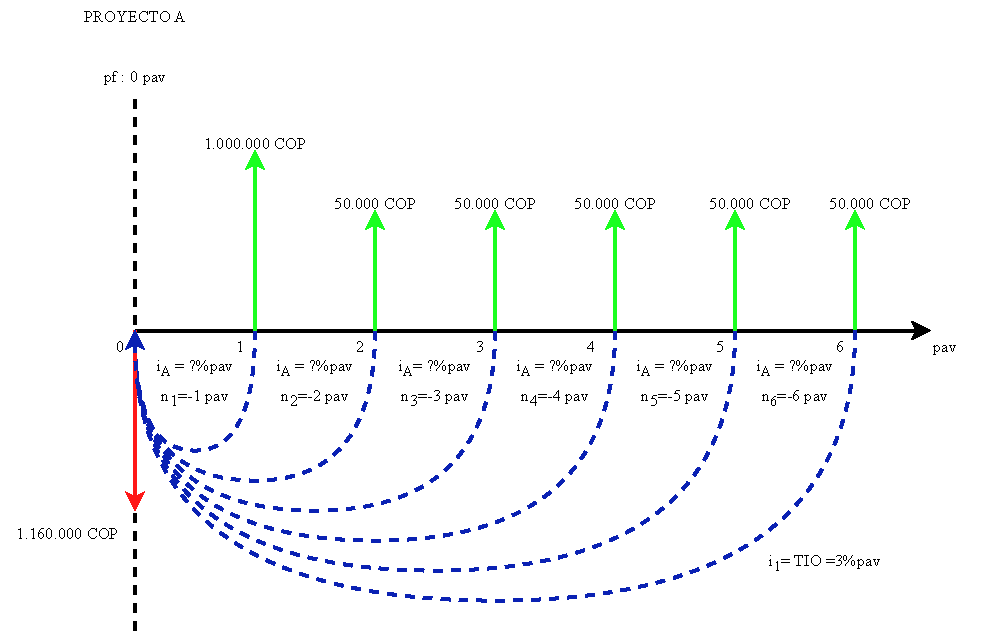
\includegraphics[scale=0.8]{ejemplos/2/Graf1Ej2Cap11.pdf} }                                                                                                \\
		\multicolumn{3}{|c|}{$ $}                                                                                                                                              \\
		\hline
		\multicolumn{3}{|c|}{$ $}                                                                                                                                              \\
		\multicolumn{3}{|c|}{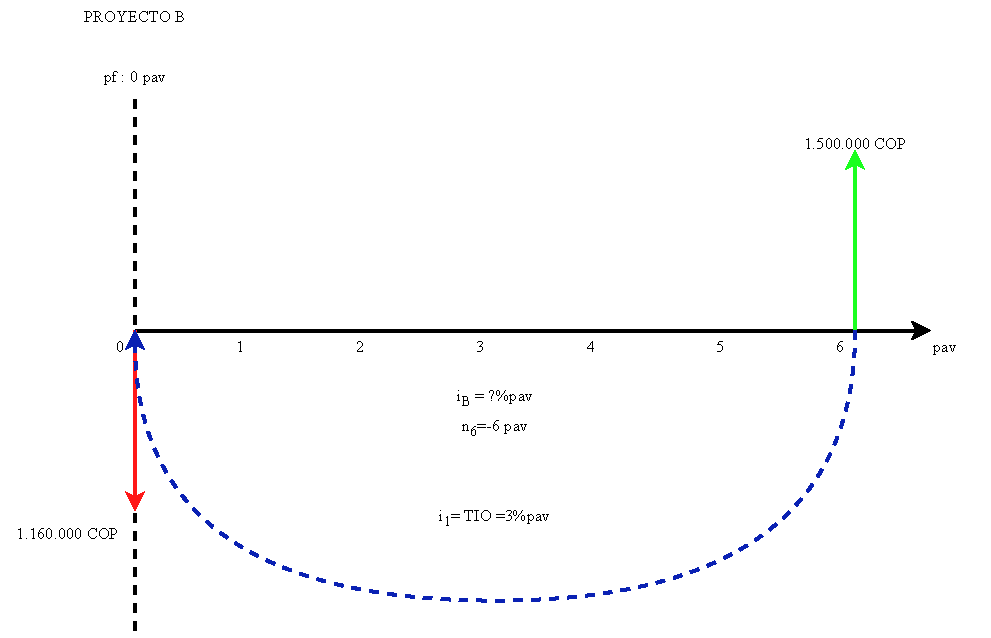
\includegraphics[scale=0.8]{ejemplos/2/Graf2Ej2Cap11.pdf} }

		\\\hline
		%%%%%%%%%%%%% FIN INSERCIÓN DE IMAGEN
		%%%%%FIN FLUJO DE CAJA



		%%%%% INICIO DECLARACIÓN FORMULAS
		%%%%%%%%%%% INICIO TITULO
		\rowcolor[HTML]{FFB183}
		\multicolumn{3}{|c|}{\cellcolor[HTML]{FFB183}\textbf{4. Declaración de fórmulas}}                                                                                      \\ \hline
		%%%%%%%%%%% FIN TITULO
		%%%%%%%%%%% INICIO MATEMÁTICAS
		\multicolumn{3}{|c|} {VPN =	$\sum F_{n}(1+i)^{-n}$   Valor presente neto.}                                                                                             \\ \hline

		%%%%%%%%%% FIN MATEMÁTICAS
		%%%%%% INICIO DESARROLLO MATEMÁTICO
		\rowcolor[HTML]{FFB183}
		%%%%%%%%%%INICIO TITULO
		\multicolumn{3}{|c|}{\cellcolor[HTML]{FFB183}\textbf{5. Desarrollo matemático}}                                                                                        \\ \hline
		%%%%%%%%%% FIN TITULO
		%%%%%%%%%% INICIO MATEMÁTICAS
		\multicolumn{3}{|c|}{$ \text{Análisis usando el VPN:} $}                                                                                                               \\
		\multicolumn{3}{|c|}{$ VPN(A) = -1\text{.}160\text{.}000\text{ COP} + 1\text{.}000\text{.}000\text{ COP}(1+0.03)^{-1} +$}                                              \\ \multicolumn{3}{|c|}{$50\text{.}000\text{ COP}(1+0.03)^{-2} + 50\text{.}000\text{ COP}(1+0.03)^{-3} + 50\text{.}000\text{ COP}(1+0.03)^{-4} $} \\
		\multicolumn{3}{|c|}{$ + 50\text{.}000\text{ COP}(1+0.03)^{-5} + 50\text{.}000\text{ COP}(1+0.03)^{-6} = 33\text{.}189.67\text{ COP.}$}                                \\
		\multicolumn{3}{|c|}{$ VPN(B) =- 1\text{.}160\text{.}000 \text{ COP} +  1\text{.}500\text{.}000(1+0.03)^{-6} = 96\text{.}226,38 \text{ COP.} $}                        \\
		\multicolumn{3}{|c|}{ $ \text{Análisis usando la TIR: } $}                                                                                                             \\
		\multicolumn{3}{|c|}{$ \text{Para calcular la TIR del proyecto A hacemos que VPN(A)=0 y dejamos la tasa como incógnita:}  $}                                           \\
		\multicolumn{3}{|c|}{$ VPN(A) = -1\text{.}160\text{.}000\text{ COP} + 1\text{.}000\text{.}000\text{ COP}(1+i_{A})^{-1} +$}                                             \\ \multicolumn{3}{|c|}{$50\text{.}000\text{ COP}(1+i_{A})^{-2} + 50\text{.}000\text{ COP}(1+i_{A})^{-3} + 50\text{.}000\text{ COP}(1+i_{A})^{-4} $} \\
		\multicolumn{3}{|c|}{$ + 50\text{.}000\text{ COP}(1+i_{A})^{-5} + 50\text{.}000\text{ COP}(1+i_{A})^{-6} = 0$}                                                         \\
		\multicolumn{3}{|c|}{$ \text{La solución manual requiere usar la interpolación, dando como resultado: } $}                                                             \\
		\multicolumn{3}{|c|}{$ i_{A} = TIR_{A} = 4.91\% pav$}                                                                                                                  \\
		\multicolumn{3}{|c|}{$ \text{Para calcular la TIR del proyecto B hacemos que VPN(B)=0 y dejamos la tasa como incógnita:}  $}                                           \\
		\multicolumn{3}{|c|}{$ VPN(B) =- 1\text{.}160\text{.}000 \text{ COP} +         1\text{.}500\text{.}000(1+i_{B})^{-6} = 0  $}                                           \\
		\multicolumn{3}{|c|}{$ \text{La solución manual requiere usar la interpolación, dando como resultado: } $}                                                             \\
		\multicolumn{3}{|c|}{$ i_{B} = TIR_{B} = 4.38\% pav$}                                                                                                                  \\

		\hline

		%%%%%%%%%% FIN MATEMÁTICAS
		%%%%%% FIN DESARROLLO MATEMÁTICO
		%%%%%% INICIO RESPUESTA
		\rowcolor[HTML]{FFB183}
		%%%%%%%%%%INICIO TITULO
		\multicolumn{3}{|c|}{\cellcolor[HTML]{FFB183}\textbf{6. Respuesta}}                                                                                                    \\ \hline
		%%%%%%%%%% FIN TITULO
		%%%%%%%%%% INICIO RESPUESTA MATEMÁTICA

		\multicolumn{3}{|c|}{ \text{El análisis usando el VPN indica que es mejor el proyecto B puesto que VPN(B)>VPN(A)} }                                                    \\
		\multicolumn{3}{|c|}{\text{El análisis usando la TIR indica que es mejor el proyecto A puesto que TIR(A)>TIR(B)}}                                                      \\
		\hline
		%%%%%%%%%% FIN MATEMÁTICAS
		%%%%%% FIN RESPUESTA
	\end{longtable}
	%Se crean dos lineas en blanco para que no quede el siguiente texto tan pegado
	%\newline \newline %USARLO SI CREES QUE ES NECESARIO
\end{center}
%%%%%%%%%%%%%%%%%%%%%%%%%%FIN EJERCICIO 2 %%%%%%%%%%%%%%%%%%%%%%%%%%%
